\mySection{14.5 The Friedman Test}
%-------------- start slide -------------------------------%{{{ 14.5
\begin{frame}{The Friedman Test}
	\begin{itemize}
		\item[] What is the nonparametric counterpart for the two-way ANOVA?
		\bigskip
		\item[Setup] Suppose that $k\ge 2$ independent sample of size $n_1,\cdots,n_k$ are drawn from $k$
		\begin{center}
			\textcolor{yellow}{identically shaped and scaled pdfs,}\\
			\textcolor{yellow}{except for possibly different medians.}
		\end{center}
		\item[] Assume that $ n_1=\cdots=n_k$.
		\item[] Samples can be further partitioned into $b$ blocks.
		\item[] Let $\widetilde{\mu}_1,\cdots,\widetilde{\mu}_k$ be the medians.
		\bigskip
		\item[Test] $H_0:\widetilde{\mu}_1=\widetilde{\mu}_2=\cdots=\widetilde{\mu}_k$ vs. $ H_1:$ not all the $\widetilde{\mu}_i$'s are equal.
		\bigskip
		\item[Remark] This is the test for median not mean, but if pdfs are symmetric, they are the same.
	\end{itemize}
\end{frame}
%-------------- end slide -------------------------------%}}}
%-------------- start slide -------------------------------%{{{ 1
\begin{frame}[fragile]
	\begin{itemize}
		\item[] \textcolor{yellow}{The Friedman Test Statistic}:
		\item[] Reject $H_0$ at the $\alpha$ level if
			\begin{align*}
				G = \frac{12}{bk(k+1)}\sum_{j=1}^k R_{\cdot j}^2  - 3b(k+1) \ge \chi_{1-\alpha,k-1}^2.
			\end{align*}
		\item[] where $R_{\cdot j}$ is the within-block ranks.
	\end{itemize}
\end{frame}
%-------------- end slide -------------------------------%}}}
%-------------- start slide -------------------------------%{{{ 1
\begin{frame}[fragile]
\begin{itemize}
	\item[E.g.] Baseball ...
	\begin{center}
	Test if $H_0:\widetilde{\mu}_{\text{Narrow}} = \widetilde{\mu}_{\text{Wide}}$	at $\alpha=0.01$
	\bigskip

	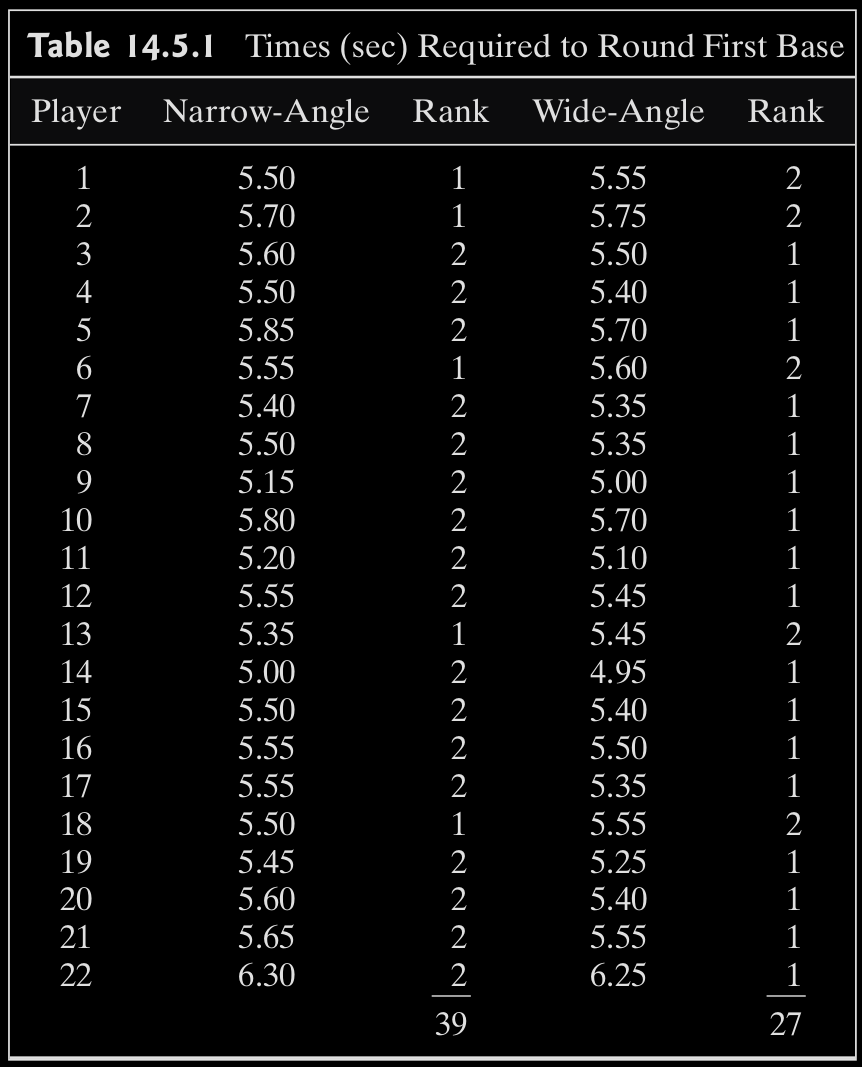
\includegraphics[scale=0.18]{Codes/Table14-5-1.png}
	\end{center}
\end{itemize}
\end{frame}
%-------------- end slide -------------------------------%}}}
%-------------- start slide -------------------------------%{{{ 1
\begin{frame}[fragile]
\begin{itemize}
	\item[Sol.] $k=2$,  $b=22$
	\bigskip
	\item[] Compute the rank within each block (see the previous table)
	\bigskip
	\item[] Compute the g statistic:
	\begin{align*}
		g=\frac{12}{22\times 2 \times (2+1)} \left[39^2+27^2\right] - 3 \times 22 \times (2+1) = \frac{72}{11}\approx 6.54.
		% sage
    %
		% 12/(22* 2 * (2+1)) *( 39^2+27^2 ) - 3 * 22 * (2+1)
    %
	\end{align*}
	\bigskip
	\item[] Critical region is
	\begin{align*}
		C = \left\{ g: g\ge \chi_{0.95,1}^2 = 3.84\right\}.
	\end{align*}
	\item[] The $p$-value is
		 \begin{align*}
			 \bbP\left(\chi_1^2 \ge \frac{72}{11}\right) = 0.01051525.
       %
			 % 1-pchisq(72/11, 1)
       %
		\end{align*}
	\item[] Conclusion: Reject. \myQED
\end{itemize}
\end{frame}
%-------------- end slide -------------------------------%}}}
%-------------- start slide -------------------------------%{{{ 1
\begin{frame}[fragile]
	R Code for this problem:
\bigskip
\begin{lstlisting}
C1 <- c(
5.50, 5.70, 5.60, 5.50, 5.85, 5.55, 5.40, 5.50, 5.15, 5.80, 5.20,
5.55, 5.35, 5.00, 5.50, 5.55, 5.55, 5.50, 5.45, 5.60, 5.65, 6.30)
C2 <- c(
5.55, 5.75, 5.50, 5.40, 5.70, 5.60, 5.35, 5.35, 5.00, 5.70, 5.10,
5.45, 5.45, 4.95, 5.40, 5.50, 5.35, 5.55, 5.25, 5.40, 5.55, 6.25)
angles <- matrix(
	cbind(C1, C2),
	nrow = 22,
	byrow = FALSE,
	dimnames = list(1:22, c("Narrow", "Wide"))
)
friedman.test(angles)
\end{lstlisting}
\end{frame}
%-------------- end slide -------------------------------%}}}
%-------------- start slide -------------------------------%{{{ 1
\begin{frame}[fragile]

Here is the output:
\bigskip
\begin{lstlisting}
	> C1 <- c(
+ 5.50, 5.70, 5.60, 5.50, 5.85, 5.55, 5.40, 5.50, 5.15, 5.80, 5.20,
+ 5.55, 5.35, 5.00, 5.50, 5.55, 5.55, 5.50, 5.45, 5.60, 5.65, 6.30)
> C2 <- c(
+ 5.55, 5.75, 5.50, 5.40, 5.70, 5.60, 5.35, 5.35, 5.00, 5.70, 5.10,
+ 5.45, 5.45, 4.95, 5.40, 5.50, 5.35, 5.55, 5.25, 5.40, 5.55, 6.25)
> angles <- matrix(
+ cbind(C1, C2),
+ nrow = 22,
+ byrow = FALSE,
+ dimnames = list(1:22, c("Narrow", "Wide"))
+ )
> friedman.test(angles)

        Friedman rank sum test

data:  angles
Friedman chi-squared = 6.5455, df = 1, p-value = 0.01052
\end{lstlisting}
\end{frame}
%-------------- end slide -------------------------------%}}}
